\section{Voxel Ray Differentials}

\subsection{Signed Distance Function and Trilinear Interpolation}
Our discrete Signed Distance Function is defined by trilinear filtering over discrete grid values. To calculate the value of the Signed Distance Function given a world position, we first have to project the world position to the local voxel grid. This can be done using the following equation to convert the world position $P_{w}$ into a voxel gird coordinate $P_{grid} \in [0, V_{resolution}]$.
\begin{equation}
P_{grid} = V_{resolution} \left(\frac{\left(P_{w} - V_{origin}\right)}{2V_{scale}}  + \begin{pmatrix}\frac{1}{2} & \frac{1}{2} & \frac{1}{2}\end{pmatrix}^T \right) 
\end{equation}
$V_{origin}$ and $V_{scale}$ represent the origin and the scale of the voxel grid, $V_{resolution}$ is its resolution.

For performing the trinilear interpolation, the 8 neighbor cells of the specific position have to be obtained. The filter weight $t$, respective to lowest cell, has to be calculated.

\begin{figure}[H]
	\caption{Trilinear filter weight $t$ to weight the 8 respective neighbor cells}
	\centering
	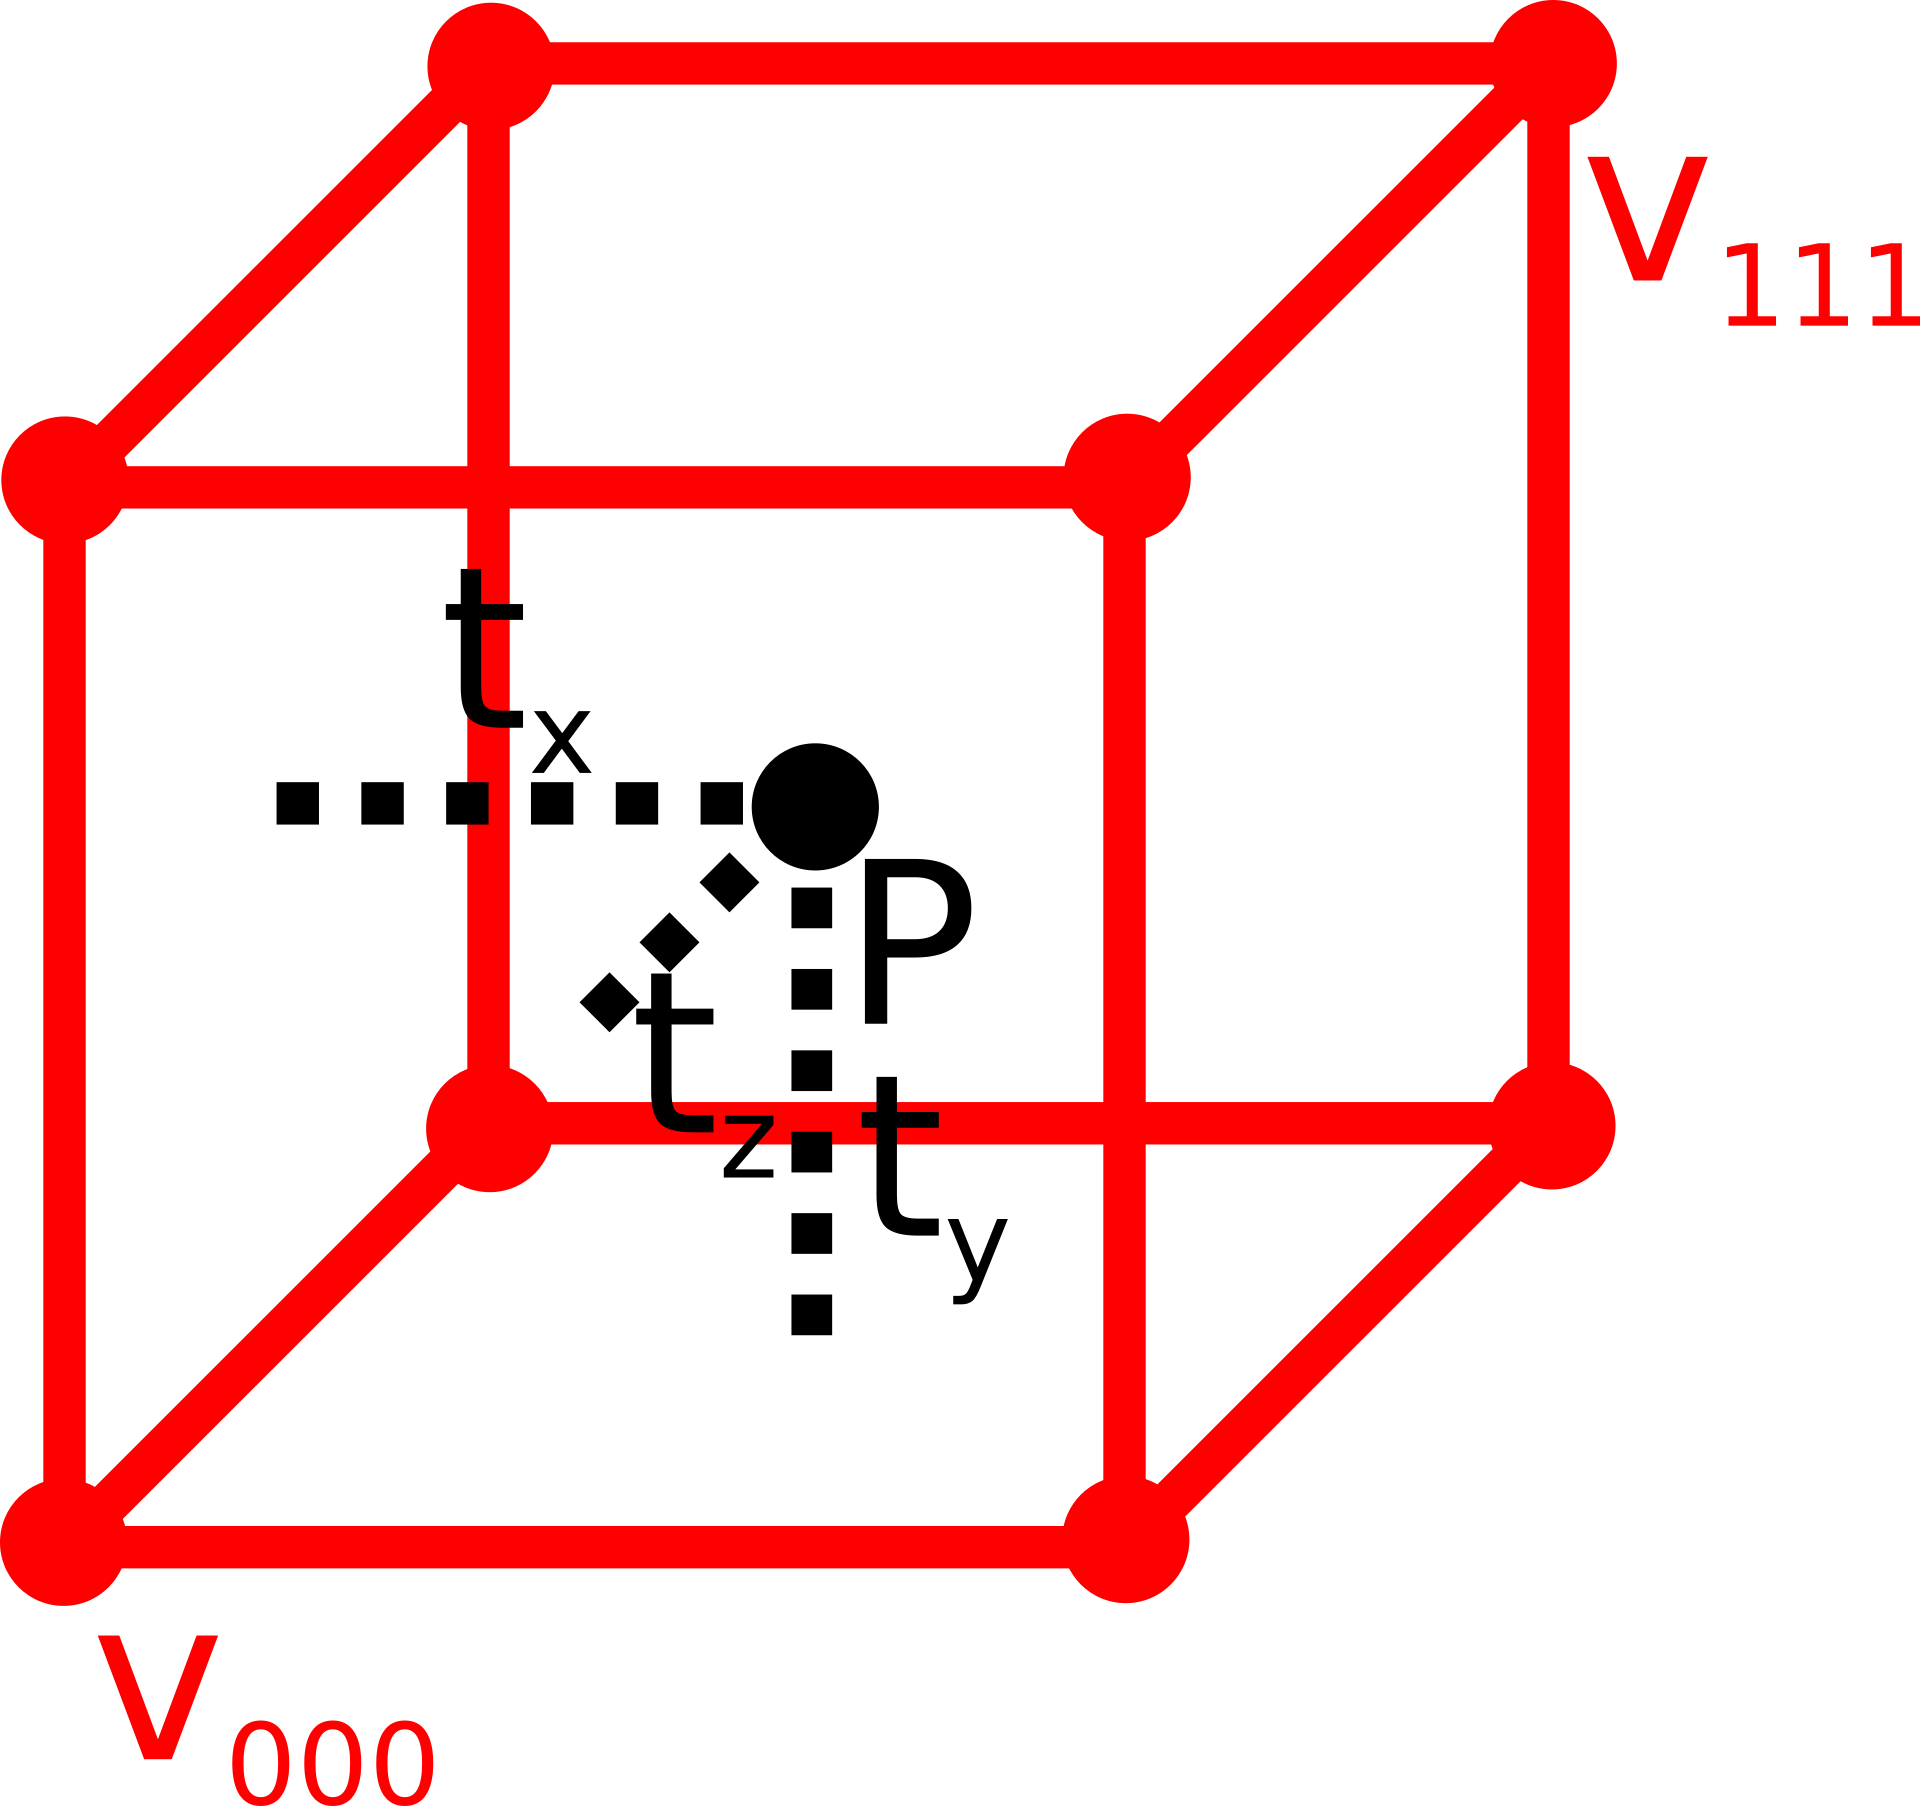
\includegraphics[width=10em]{images/trilinear_filter_weight}
\end{figure}
\begin{equation}
t = P_{grid} - P_{000}
\end{equation}
Since the width of a cell is 1, no division has to be done.

The final step is to build the filter matrix $T$ and calculate its dot product with the 8 neighbor cells. This yields the interpolated value at $P_{grid}$, the value of the Signed Distance Function.

\begin{equation}
T =
\begin{pmatrix}
(1 - t_x) (1 - t_y) (1 - t_z) \\
t_x (1 - t_y) (1 - t_z) \\
(1 - t_x) t_y (1 - t_z) \\
(1 - t_x) (1 - t_y) t_z \\
t_x t_y (1 - t_z) \\
t_x (1 - t_y) t_z \\
(1 - t_x) t_y t_z \\
t_x t_y t_z
\end{pmatrix}	
V =
\begin{pmatrix}
v_{000} \\
v_{100} \\
v_{010} \\
v_{001} \\
v_{110} \\
v_{101} \\
v_{011} \\
v_{111} 
\end{pmatrix}
, trilinear(t, V) = T \cdot V
\end{equation}

\begin{equation}
SDF(P) = trilinear(t_P, V_{sdf})
\end{equation}

\subsection{Surface Normal}

The surface of the Signed Distance Function is defined as the set of points where the Signed Distance Function yields 0.
\begin{equation}
S_{surface} = \{P \in \mathbb{R}^3 \mid SDF(P) = 0\}
\end{equation}
For $P \in S_{surface}$, the surface normal $N$ is defined as the gradient of the Signed Distance Field.

\begin{equation}
n_{surface} = \nabla SDF = 
\begin{pmatrix}
\pardiff{trilinear(t_P, V_{sdf})}{x_{w}} \newlinell
\pardiff{trilinear(t_P, V_{sdf})}{y_{w}} \newlinell
\pardiff{trilinear(t_P, V_{sdf})}{z_{w}}
\end{pmatrix}
\end{equation}
$\partial x_{w}$, $\partial y_{w}$ and $\partial z_{w}$ denotes the differential in world coordinates, a change in the x, y and z-axis. To calculate the gradient of the Signed Distance Function, the trilinear interpolation has to be differentiated. For the x-direction, the differential of the trilinear filter weight $t$ is a constant value depending on the scale and resolution of the grid

\begin{equation}
\pardiff{P_w}{x_w} = 
\begin{pmatrix}
1 & 0 & 0
\end{pmatrix}^T
\qquad
\pardiff{t}{x_w} = 
\frac{V_{resolution}}{2V_{scale}}
\begin{pmatrix}
1 & 0 & 0
\end{pmatrix}^T.
\end{equation}
This results in the following equation for the differential of the trilinear interpolation in x-direction.

\begin{equation}
\pardiff{trilinear(t_P, V_{sdf})}{x_{w}} = 
\frac{V_{resolution}}{2V_{scale}}
V_{sdf} \cdot
\begin{pmatrix}
-(1 - t_y) (1 - t_z) \newlinel
(1 - t_y) (1 - t_z) \newlinel
-t_y (1 - t_z) \newlinel
-(1 - t_y) t_z \newlinel
t_y (1 - t_z) \newlinel
(1 - t_y) t_z \newlinel
-t_y t_z \newlinel
t_y t_z
\end{pmatrix}
\end{equation}
A similar expression can be derived for the y and z-direction. Final normalization results in the surface normal

\begin{equation}
N_{surface} = \frac{n_{surface}}{\left(n_{surface} \cdot n_{surface}\right)^{1/2}} .
\end{equation}

\subsubsection{Surface Normal Differentials}
To use ray differentials with voxel based objects, the surface normal has to be differentiated by the image plane coordinates $x$ and $y$.
\begin{equation}
\pardiffx{n_{surface}} = 
\begin{pmatrix}
\pardiffsq{trilinear(t_P, V_{sdf})}{x_{w}}{x} \newlinell
\pardiffsq{trilinear(t_P, V_{sdf})}{y_{w}}{x} \newlinell
\pardiffsq{trilinear(t_P, V_{sdf})}{z_{w}}{x}
\end{pmatrix}
\qquad
\pardiffy{n_{surface}} = 
\begin{pmatrix}
\pardiffsq{trilinear(t_P, V_{sdf})}{x_{w}}{y} \newlinell
\pardiffsq{trilinear(t_P, V_{sdf})}{y_{w}}{y} \newlinell
\pardiffsq{trilinear(t_P, V_{sdf})}{z_{w}}{y}
\end{pmatrix}
\end{equation}
The differential of the interpolation weight $t$ by the image plane coordinates based on the ray differential positions $\pardiffx{P}$ and $\pardiffy{P}$ is
\begin{equation}
\pardiff{t}{x} = \frac{V_{resolution}}{2V_{scale}} \pardiff{P}{x}
\qquad
\pardiff{t}{y} = \frac{V_{resolution}}{2V_{scale}} \pardiff{P}{y}.
\end{equation}
This yields the following term for the x-coordinate of the $\partial x$ normal differential $\pardiffx{n_{surface}}$
\begin{equation}
\pardiffsq{trilinear(t_P, V_{sdf})}{x_{w}}{x} = 
\left(\frac{V_{resolution}}{2V_{scale}}\right)^2
V_{sdf}
\cdot
\left(
\begin{pmatrix}
\pardiffx{P_y} (1 - t_z) \newlinel
-\pardiffx{P_y} (1 - t_z) \newlinel
-\pardiffx{P_y} (1 - t_z) \newlinel
\pardiffx{P_y} t_z \newlinel
\pardiffx{P_y} (1 - t_z) \newlinel
-\pardiffx{P_y} t_z \newlinel
-\pardiffx{P_y} t_z \newlinel
\pardiffx{P_y} t_z
\end{pmatrix}
+
\begin{pmatrix}
(1 - t_y) \pardiffx{P_z} \newlinel
-(1 - t_y) \pardiffx{P_z} \newlinel
t_y \pardiffx{P_z} \newlinel
-(1 - t_y) \pardiffx{P_z} \newlinel
-t_y \pardiffx{P_z} \newlinel
(1 - t_y) \pardiffx{P_z} \newlinel
-t_y \pardiffx{P_z} \newlinel
t_y \pardiffx{P_z}
\end{pmatrix}
\right).
\end{equation}
All other 5 components can be derived regarding this expression. To retrieve the normalized normal differential, the normalization term has to be derived to receive
\begin{equation}
\pardiffx{N} = \frac{(n \cdot n) \pardiffx{n} - (n \cdot \pardiffx{n}) n}{(n \cdot n)^{3/2}}
\end{equation}

\subsection {Shading Normal}
Using surface normals produces hard edges on voxel borders which reveals the block structure. To avoid this problem, trilinear interpolation of the surface normals can be applied to receive a smooth normal at a given point.
\begin{equation}
n = trilinear(t_p, V_{N_{surface}})
\end{equation}
where $V_{N_{surface}}$ is an 8-compoment vector consisting of the surface normals of the 8 neighbor cells of the respective position.
\subsubsection {Shading Normal Differential}
The differential of the shading normal requires the differential of the trilinear equation. For the $\partial x$ differential this would be
\begin{equation}
\pardiffx{n} = \pardiffx{trilinear(t_p, V_{N_{surface}})} = \pardiffx{T} \cdot V_{N_{surface}}
\end{equation}

\begin{equation}
\begin{aligned}
\pardiffx{T} &=
\begin{pmatrix}
\left(-\pardiffx{t_x}\right) (1 - t_y) (1 - t_z) \newlinel
\pardiffx{t_x} (1 - t_y) (1 - t_z) \newlinel
\left(-\pardiffx{t_x}\right) t_y (1 - t_z) \newlinel
\left(-\pardiffx{t_x}\right) (1 - t_y) t_z \newlinel
\pardiffx{t_x} t_y (1 - t_z) \newlinel
\pardiffx{t_x} (1 - t_y) t_z \newlinel
\left(-\pardiffx{t_x}\right) t_y t_z \newlinel
\pardiffx{t_x} t_y t_z
\end{pmatrix}
+
\begin{pmatrix}
(1 - t_x) \left(-\pardiffx{t_y}\right) (1 - t_z) \newlinel
t_x \left(-\pardiffx{t_y}\right) (1 - t_z) \newlinel
(1 - t_x) \pardiffx{t_y} (1 - t_z) \newlinel
(1 - t_x) \left(-\pardiffx{t_y}\right) t_z \newlinel
t_x \pardiffx{t_y} (1 - t_z) \newlinel
t_x \left(-\pardiffx{t_y}\right) t_z \newlinel
(1 - t_x) \pardiffx{t_y} t_z \newlinel
t_x \pardiffx{t_y} t_z
\end{pmatrix}
\\
&+
\begin{pmatrix}
(1 - t_x) (1 - t_y) \left(-\pardiffx{t_z}\right) \newlinel
t_x (1 - t_y) \left(-\pardiffx{t_z}\right) \newlinel
(1 - t_x) t_y \left(-\pardiffx{t_z}\right) \newlinel
(1 - t_x) (1 - t_y) \pardiffx{t_z} \newlinel
t_x t_y \left(-\pardiffx{t_z}\right) \newlinel
t_x (1 - t_y) \pardiffx{t_z} \newlinel
(1 - t_x) t_y \pardiffx{t_z} \newlinel
t_x t_y \pardiffx{t_z}
\end{pmatrix}
\end{aligned}
\end{equation}

\subsection{New Section}
1D kernel with kernel width $n$
\begin{equation}
f(v_0, \dots, v_{n-1}, t)
\end{equation}
Linear filter kernel example
\begin{equation}
f(v_0, v_1, t) = (1 - t) v_0 + t v_1
\end{equation}
Applying kernel with width $2$ to 3D voxel grid
\begin{equation}
%f(f(f(v0, v1, t_x(P)), f(v2, v3, t_x(P)), t_y(P)), f(f(v4, v5, t_x(P)), f(v6, v7, t_x(P)), t_y(P)), t_z(P))
v(t) = f
\begin{pmatrix}
f 
\begin{pmatrix}
f(v0, v1, t_x), \\
f(v2, v3, t_x), \\
t_y
\end{pmatrix}, \\[2.0em]
f
\begin{pmatrix}
f(v4, v5, t_x), \\
f(v6, v7, t_x), \\
t_y
\end{pmatrix}, \\[2.0em]
t_z
\end{pmatrix}
\end{equation}
\begin{equation}
SDF(P) = v(t(P))
\end{equation}
Normal
\begin{equation}
n = \nabla SDF = 
\begin{pmatrix}
\pardiff{SDF}{P_x} \newlinell
\pardiff{SDF}{P_y} \newlinell
\pardiff{SDF}{P_z}
\end{pmatrix}
=
\begin{pmatrix}
\pardiff{v}{t_x} \newlinell
\pardiff{v}{t_y} \newlinell
\pardiff{v}{t_z}
\end{pmatrix}
\odot
\begin{pmatrix}
\pardiff{t_x}{P_x} \newlinell
\pardiff{t_y}{P_y} \newlinell
\pardiff{t_z}{P_z}
\end{pmatrix}
=
\nabla v \odot \pardiff{t}{P}
\end{equation}
Normal Differentials
\begin{equation}
\begin{aligned}
\pardiff{n}{x} &= \pardiff{\nabla SDF}{x} = 
\begin{pmatrix}
\pardiffsq{SDF}{P_x}{x} \newlinell
\pardiffsq{SDF}{P_y}{x} \newlinell
\pardiffsq{SDF}{P_z}{x}
\end{pmatrix} \newlinell
&=
\begin{pmatrix}
\pardiffsqsame{v}{t_x} \pardiff{t_x}{P_x} \pardiff{P_x}{x} + \pardiffsq{v}{t_x}{t_y} \pardiff{t_y}{P_y} \pardiff{P_y}{x} + \pardiffsq{v}{t_x}{t_z} \pardiff{t_z}{P_z} \pardiff{P_z}{x} \newlinell
\pardiffsq{v}{t_y}{t_x} \pardiff{t_x}{P_x} \pardiff{P_x}{x} + \pardiffsqsame{v}{t_y} \pardiff{t_y}{P_y} \pardiff{P_y}{x} + \pardiffsq{v}{t_y}{t_z} \pardiff{t_z}{P_z} \pardiff{P_z}{x} \newlinell
\pardiffsq{v}{t_z}{t_x} \pardiff{t_x}{P_x} \pardiff{P_x}{x} + \pardiffsq{v}{t_z}{t_y} \pardiff{t_y}{P_y} \pardiff{P_y}{x} + \pardiffsqsame{v}{t_z} \pardiff{t_z}{P_z} \pardiff{P_z}{x}
\end{pmatrix}
\odot \pardiff{t}{P} \newlinell
&=
\begin{pmatrix}
\pardiffsqsame{v}{t_x} & \pardiffsq{v}{t_x}{t_y} & \pardiffsq{v}{t_x}{t_z} \newlinell
\pardiffsq{v}{t_y}{t_x} & \pardiffsqsame{v}{t_y} & \pardiffsq{v}{t_y}{t_z} \newlinell
\pardiffsq{v}{t_z}{t_x} & \pardiffsq{v}{t_z}{t_y} & \pardiffsqsame{v}{t_z}
\end{pmatrix}
\cdot \left( \pardiff{t}{P} \odot \pardiff{t}{P} \odot \pardiff{P}{x} \right) \newlinell
&= \Hessian(v) \cdot \left(\pardiff{t}{P} \odot \pardiff{t}{P} \odot \pardiff{P}{x} \right)
\end{aligned}
\end{equation}
